%% This style is provided for the ICSE 2015 main conference,
%% ICSE 2015 co-located events, and ICSE 2015 workshops.

%% bare_conf_ICSE15.tex
%% V1.4
%% 2014/05/22


%% This is a skeleton file demonstrating the use of IEEEtran.cls
%% (requires IEEEtran.cls version 1.7 or later) with an IEEE conference paper.
%%
%% Support sites:
%% http://www.michaelshell.org/tex/ieeetran/
%% http://www.ctan.org/tex-archive/macros/latex/contrib/IEEEtran/
%% and
%% http://www.ieee.org/

%%*************************************************************************
%% Legal Notice:
%% This code is offered as-is without any warranty either expressed or
%% implied; without even the implied warranty of MERCHANTABILITY or
%% FITNESS FOR A PARTICULAR PURPOSE!
%% User assumes all risk.
%% In no event shall IEEE or any contributor to this code be liable for
%% any damages or losses, including, but not limited to, incidental,
%% consequential, or any other damages, resulting from the use or misuse
%% of any information contained here.
%%
%% All comments are the opinions of their respective authors and are not
%% necessarily endorsed by the IEEE.
%%
%% This work is distributed under the LaTeX Project Public License (LPPL)
%% ( http://www.latex-project.org/ ) version 1.3, and may be freely used,
%% distributed and modified. A copy of the LPPL, version 1.3, is included
%% in the base LaTeX documentation of all distributions of LaTeX released
%% 2003/12/01 or later.
%% Retain all contribution notices and credits.
%% ** Modified files should be clearly indicated as such, including  **
%% ** renaming them and changing author support contact information. **
%%
%% File list of work: IEEEtran.cls, IEEEtran_HOWTO.pdf, bare_adv.tex,
%%                    bare_conf.tex, bare_jrnl.tex, bare_jrnl_compsoc.tex
%%*************************************************************************

% *** Authors should verify (and, if needed, correct) their LaTeX system  ***
% *** with the testflow diagnostic prior to trusting their LaTeX platform ***
% *** with production work. IEEE's font choices can trigger bugs that do  ***
% *** not appear when using other class files.                            ***
% The testflow support page is at:
% http://www.michaelshell.org/tex/testflow/



% Note that the a4paper option is mainly intended so that authors in
% countries using A4 can easily print to A4 and see how their papers will
% look in print - the typesetting of the document will not typically be
% affected with changes in paper size (but the bottom and side margins will).
% Use the testflow package mentioned above to verify correct handling of
% both paper sizes by the user's LaTeX system.
%
% Also note that the "draftcls" or "draftclsnofoot", not "draft", option
% should be used if it is desired that the figures are to be displayed in
% draft mode.
%
\documentclass[conference]{IEEEtran}
% \documentclass[draft]{IEEEtran}
%
% If IEEEtran.cls has not been installed into the LaTeX system files,
% manually specify the path to it like:
% \documentclass[conference]{../sty/IEEEtran}





% Some very useful LaTeX packages include:
% (uncomment the ones you want to load)


% *** MISC UTILITY PACKAGES ***
%
%\usepackage{ifpdf}
% Heiko Oberdiek's ifpdf.sty is very useful if you need conditional
% compilation based on whether the output is pdf or dvi.
% usage:
% \ifpdf
%   % pdf code
% \else
%   % dvi code
% \fi
% The latest version of ifpdf.sty can be obtained from:
% http://www.ctan.org/tex-archive/macros/latex/contrib/oberdiek/
% Also, note that IEEEtran.cls V1.7 and later provides a builtin
% \ifCLASSINFOpdf conditional that works the same way.
% When switching from latex to pdflatex and vice-versa, the compiler may
% have to be run twice to clear warning/error messages.


%Todd added for fractions
\usepackage{xfrac}
%Todd added for strike-outs
\usepackage{ulem}
%Todd added for mutlirow tables
\usepackage{multirow}
%Todd added for graphics generation
\usepackage{tikz}
\usetikzlibrary{"automata"}
%Todd added for cross referencing verbatim listings
\usepackage{listings}
%Todd added for psuedocode listings
\usepackage{algpseudocode}



% *** CITATION PACKAGES ***
%
%\usepackage{cite}
% cite.sty was written by Donald Arseneau
% V1.6 and later of IEEEtran pre-defines the format of the cite.sty package
% \cite output to follow that of IEEE. Loading the cite package will
% result in citation numbers being automatically sorted and properly
% "compressed/ranged". e.g., [1], [9], [2], [7], [5], [6] without using
% cite.sty will become [1], [2], [5]--[7], [9] using cite.sty. cite.sty's
% \cite will automatically add leading space, if needed. Use cite.sty's
% noadjust option (cite.sty V3.8 and later) if you want to turn this off.
% cite.sty is already installed on most LaTeX systems. Be sure and use
% version 4.0 (2003-05-27) and later if using hyperref.sty. cite.sty does
% not currently provide for hyperlinked citations.
% The latest version can be obtained at:
% http://www.ctan.org/tex-archive/macros/latex/contrib/cite/
% The documentation is contained in the cite.sty file itself.






% *** GRAPHICS RELATED PACKAGES ***
%
\ifCLASSINFOpdf
  \usepackage[pdftex]{graphicx}
  % declare the path(s) where your graphic files are
  % \graphicspath{{../pdf/}{../jpeg/}}
  % and their extensions so you won't have to specify these with
  % every instance of \includegraphics
  \DeclareGraphicsExtensions{.pdf,.jpeg,.png}
\else
  % or other class option (dvipsone, dvipdf, if not using dvips). graphicx
  % will default to the driver specified in the system graphics.cfg if no
  % driver is specified.
  % \usepackage[dvips]{graphicx}
  % declare the path(s) where your graphic files are
  % \graphicspath{{../eps/}}
  % and their extensions so you won't have to specify these with
  % every instance of \includegraphics
  % \DeclareGraphicsExtensions{.eps}
\fi
% graphicx was written by David Carlisle and Sebastian Rahtz. It is
% required if you want graphics, photos, etc. graphicx.sty is already
% installed on most LaTeX systems. The latest version and documentation can
% be obtained at:
% http://www.ctan.org/tex-archive/macros/latex/required/graphics/
% Another good source of documentation is "Using Imported Graphics in
% LaTeX2e" by Keith Reckdahl which can be found as epslatex.ps or
% epslatex.pdf at: http://www.ctan.org/tex-archive/info/
%
% latex, and pdflatex in dvi mode, support graphics in encapsulated
% postscript (.eps) format. pdflatex in pdf mode supports graphics
% in .pdf, .jpeg, .png and .mps (metapost) formats. Users should ensure
% that all non-photo figures use a vector format (.eps, .pdf, .mps) and
% not a bitmapped formats (.jpeg, .png). IEEE frowns on bitmapped formats
% which can result in "jaggedy"/blurry rendering of lines and letters as
% well as large increases in file sizes.
%
% You can find documentation about the pdfTeX application at:
% http://www.tug.org/applications/pdftex





% *** MATH PACKAGES ***
%
%\usepackage[cmex10]{amsmath}
% A popular package from the American Mathematical Society that provides
% many useful and powerful commands for dealing with mathematics. If using
% it, be sure to load this package with the cmex10 option to ensure that
% only type 1 fonts will utilized at all point sizes. Without this option,
% it is possible that some math symbols, particularly those within
% footnotes, will be rendered in bitmap form which will result in a
% document that can not be IEEE Xplore compliant!
%
% Also, note that the amsmath package sets \interdisplaylinepenalty to 10000
% thus preventing page breaks from occurring within multiline equations. Use:
%\interdisplaylinepenalty=2500
% after loading amsmath to restore such page breaks as IEEEtran.cls normally
% does. amsmath.sty is already installed on most LaTeX systems. The latest
% version and documentation can be obtained at:
% http://www.ctan.org/tex-archive/macros/latex/required/amslatex/math/





% *** SPECIALIZED LIST PACKAGES ***
%
%\usepackage{algorithmic}
% algorithmic.sty was written by Peter Williams and Rogerio Brito.
% This package provides an algorithmic environment fo describing algorithms.
% You can use the algorithmic environment in-text or within a figure
% environment to provide for a floating algorithm. Do NOT use the algorithm
% floating environment provided by algorithm.sty (by the same authors) or
% algorithm2e.sty (by Christophe Fiorio) as IEEE does not use dedicated
% algorithm float types and packages that provide these will not provide
% correct IEEE style captions. The latest version and documentation of
% algorithmic.sty can be obtained at:
% http://www.ctan.org/tex-archive/macros/latex/contrib/algorithms/
% There is also a support site at:
% http://algorithms.berlios.de/index.html
% Also of interest may be the (relatively newer and more customizable)
% algorithmicx.sty package by Szasz Janos:
% http://www.ctan.org/tex-archive/macros/latex/contrib/algorithmicx/




% *** ALIGNMENT PACKAGES ***
%
%\usepackage{array}
% Frank Mittelbach's and David Carlisle's array.sty patches and improves
% the standard LaTeX2e array and tabular environments to provide better
% appearance and additional user controls. As the default LaTeX2e table
% generation code is lacking to the point of almost being broken with
% respect to the quality of the end results, all users are strongly
% advised to use an enhanced (at the very least that provided by array.sty)
% set of table tools. array.sty is already installed on most systems. The
% latest version and documentation can be obtained at:
% http://www.ctan.org/tex-archive/macros/latex/required/tools/


%\usepackage{mdwmath}
%\usepackage{mdwtab}
% Also highly recommended is Mark Wooding's extremely powerful MDW tools,
% especially mdwmath.sty and mdwtab.sty which are used to format equations
% and tables, respectively. The MDWtools set is already installed on most
% LaTeX systems. The lastest version and documentation is available at:
% http://www.ctan.org/tex-archive/macros/latex/contrib/mdwtools/


% IEEEtran contains the IEEEeqnarray family of commands that can be used to
% generate multiline equations as well as matrices, tables, etc., of high
% quality.


%\usepackage{eqparbox}
% Also of notable interest is Scott Pakin's eqparbox package for creating
% (automatically sized) equal width boxes - aka "natural width parboxes".
% Available at:
% http://www.ctan.org/tex-archive/macros/latex/contrib/eqparbox/





% *** SUBFIGURE PACKAGES ***
%\usepackage[tight,footnotesize]{subfigure}
% subfigure.sty was written by Steven Douglas Cochran. This package makes it
% easy to put subfigures in your figures. e.g., "Figure 1a and 1b". For IEEE
% work, it is a good idea to load it with the tight package option to reduce
% the amount of white space around the subfigures. subfigure.sty is already
% installed on most LaTeX systems. The latest version and documentation can
% be obtained at:
% http://www.ctan.org/tex-archive/obsolete/macros/latex/contrib/subfigure/
% subfigure.sty has been superceeded by subfig.sty.



%\usepackage[caption=false]{caption}
%\usepackage[font=footnotesize]{subfig}
% subfig.sty, also written by Steven Douglas Cochran, is the modern
% replacement for subfigure.sty. However, subfig.sty requires and
% automatically loads Axel Sommerfeldt's caption.sty which will override
% IEEEtran.cls handling of captions and this will result in nonIEEE style
% figure/table captions. To prevent this problem, be sure and preload
% caption.sty with its "caption=false" package option. This is will preserve
% IEEEtran.cls handing of captions. Version 1.3 (2005/06/28) and later
% (recommended due to many improvements over 1.2) of subfig.sty supports
% the caption=false option directly:
%\usepackage[caption=false,font=footnotesize]{subfig}
%
% The latest version and documentation can be obtained at:
% http://www.ctan.org/tex-archive/macros/latex/contrib/subfig/
% The latest version and documentation of caption.sty can be obtained at:
% http://www.ctan.org/tex-archive/macros/latex/contrib/caption/




% *** FLOAT PACKAGES ***
%
%\usepackage{fixltx2e}
% fixltx2e, the successor to the earlier fix2col.sty, was written by
% Frank Mittelbach and David Carlisle. This package corrects a few problems
% in the LaTeX2e kernel, the most notable of which is that in current
% LaTeX2e releases, the ordering of single and double column floats is not
% guaranteed to be preserved. Thus, an unpatched LaTeX2e can allow a
% single column figure to be placed prior to an earlier double column
% figure. The latest version and documentation can be found at:
% http://www.ctan.org/tex-archive/macros/latex/base/



%\usepackage{stfloats}
% stfloats.sty was written by Sigitas Tolusis. This package gives LaTeX2e
% the ability to do double column floats at the bottom of the page as well
% as the top. (e.g., "\begin{figure*}[!b]" is not normally possible in
% LaTeX2e). It also provides a command:
%\fnbelowfloat
% to enable the placement of footnotes below bottom floats (the standard
% LaTeX2e kernel puts them above bottom floats). This is an invasive package
% which rewrites many portions of the LaTeX2e float routines. It may not work
% with other packages that modify the LaTeX2e float routines. The latest
% version and documentation can be obtained at:
% http://www.ctan.org/tex-archive/macros/latex/contrib/sttools/
% Documentation is contained in the stfloats.sty comments as well as in the
% presfull.pdf file. Do not use the stfloats baselinefloat ability as IEEE
% does not allow \baselineskip to stretch. Authors submitting work to the
% IEEE should note that IEEE rarely uses double column equations and
% that authors should try to avoid such use. Do not be tempted to use the
% cuted.sty or midfloat.sty packages (also by Sigitas Tolusis) as IEEE does
% not format its papers in such ways.





% *** PDF, URL AND HYPERLINK PACKAGES ***
%
%\usepackage{url}
% url.sty was written by Donald Arseneau. It provides better support for
% handling and breaking URLs. url.sty is already installed on most LaTeX
% systems. The latest version can be obtained at:
% http://www.ctan.org/tex-archive/macros/latex/contrib/misc/
% Read the url.sty source comments for usage information. Basically,
% \url{my_url_here}.





% *** Do not adjust lengths that control margins, column widths, etc. ***
% *** Do not use packages that alter fonts (such as pslatex).         ***
% There should be no need to do such things with IEEEtran.cls V1.6 and later.
% (Unless specifically asked to do so by the journal or conference you plan
% to submit to, of course. )


% correct bad hyphenation here
\hyphenation{op-tical net-works semi-conduc-tor}


\begin{document}
%
% paper title
% can use linebreaks \\ within to get better formatting as desired
%\title{Green-Lighting Software Engineering Practicums with SEMAT Essence}
\title{Towards Generating Essence Kernels Using Genetic Algorithms}

% author names and affiliations
% use a multiple column layout for up to three different
% affiliations
%\author{\IEEEauthorblockN{Michael Shell}
%\IEEEauthorblockA{School of Electrical and\\Computer Engineering\\
%Georgia Institute of Technology\\
%Atlanta, Georgia 30332--0250\\
%Email: http://www.michaelshell.org/contact.html}
%\and
%\IEEEauthorblockN{Homer Simpson}
%\IEEEauthorblockA{Twentieth Century Fox\\
%Springfield, USA\\
%Email: homer@thesimpsons.com}
%\and
%\IEEEauthorblockN{James Kirk\\ and Montgomery Scott}
%\IEEEauthorblockA{Starfleet Academy\\
%San Francisco, California 96678-2391\\
%Telephone: (800) 555--1212\\
%Fax: (888) 555--1212}}

% conference papers do not typically use \thanks and this command
% is locked out in conference mode. If really needed, such as for
% the acknowledgment of grants, issue a \IEEEoverridecommandlockouts
% after \documentclass

% for over three affiliations, or if they all won't fit within the width
% of the page, use this alternative format:
%
\author{\IEEEauthorblockN{Todd Sedano, C\'ecile P\`eraire
}
\IEEEauthorblockA{Carnegie Mellon Unveristy \\
Silicon Valley Campus\\
Moffett Field, CA 94035, USA \\
Email: todd.sedano@sv.cmu.edu, cecile.peraire@sv.cmu.edu
}}

% use for special paper notices
%\IEEEspecialpapernotice{(Invited Paper)}

% make the title area
\maketitle

\begin{abstract}
The SEMAT community created the Essence Kernel as a unifying framework for describing and analyzing software engineering endeavors. \cite{JacobsonQueue} The Essence Kernel is based upon human experience and judgement, not empirical data. 

Background: At Carnegie Mellon University in Silicon Valley, we have collected data from masters of science in software engineering students as they complete a team-based project course as their capstone or practicum project. Each week, the team records their progress in an Essence Reflection meeting \cite{EASE2014}. This data serves as training data for evaluating the Essence Kernel and alternative candidate kernels.

Objective: Optimize candidate replacement kernels by using a fitness function based on empirical data in order to improve the Essence Kernel.

Method: Using genetic programming, the kernel genotype will be represented as a collection of linear state machines each with a collection of unique checklist items. Operations to evolve the genotypes include randomly moving checklist items, splitting states, and deleting states by moving their checklist items to other states. 

Results: Genetic programming created random candidate essence kernels that scored higher fitness scores than the original essence kernel. The purpose of this exploratory work is to show one way to generate a candidate Essence kernel directly from empirical data, not to recommend a replacement for the original Essence Kernel.

Limitations: Given the limited amount of data, the generated kernels may be over-optimized. Additional empirical data is required before recommending replacing the original kernel with a candidate kernel that fits the data.

Conclusion: The original Essence kernel is highly structured around human notions of order. Genetic Algorithms can generate candidate kernels that humans might not normally consider.
\end{abstract}

% For peer review papers, you can put extra information on the cover
% page as needed:
% \ifCLASSOPTIONpeerreview
% \begin{center} \bfseries EDICS Category: 3-BBND \end{center}
% \fi
%
% For peerreview papers, this IEEEtran command inserts a page break and
% creates the second title. It will be ignored for other modes.
\IEEEpeerreviewmaketitle

\section{Background}
The SEMAT community created Essence as a universal framework for any software engineering project. At the core of Essence is a ``kernel of widely-agreed elements'' ~\cite{JacobsonQueue}. This general kernel can theoretically support any kind of software endeavor. A software project can define its software processes by using the general kernel, extending the kernel, or defining additional practices on top of the kernel.

The Essence kernel is composed of a set of alphas, alpha states, and alpha state checklist items. The Essence kernel defines different characteristics or dimensions of a software project as an ``alpha.'' The seven alphas are \textbf{Stakeholders}, \textbf{Opportunity}, \textbf{Requirements}, \textbf{Software System}, \textbf{Team}, \textbf{Way of Working}, and \textbf{Work}. Essence decomposes each of these alphas into a set of states that represent a simple linear state machine as shown in Figure \ref{StateMachine}. For example, the \textbf{Requirements} alpha advances through the states \textit{Conceived}, \textit{Bounded}, \textit{Coherent}, \textit{Acceptable}, \textit{Addressed}, and \textit{Fulfilled.} Each state has a checklist or set of goals. To achieve a state, the project must satisfy every checklist item for that state. \cite{OMGStandard} 
 
\begin{figure}[ht]
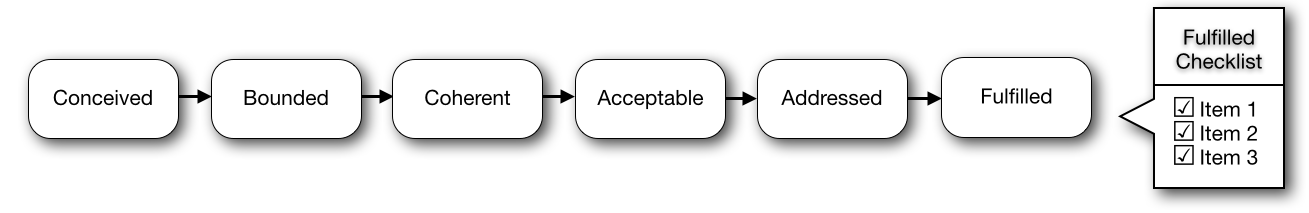
\includegraphics[scale=0.34]{kernel_images/StateMachineRequirements}
\caption{Kernel's linear state machine for Requirements alpha}\label{StateMachine}
\end{figure}


%I have finished research in evaluating the Project Monitoring and Steering approach, Green-lighting Practicum projects and compared Essence Reflection meetings to Agile Reflection meetings. For evaluating the Project Monitoring and Steering approach a two semester field study involving quantitative and qualitative data collection revealed the value of the SEMAT Essence approach for a team-based project course. \cite{ICSE2014} The Essence kernel provides mechanisms for monitoring progress, steering projects, and routine team reflection, in a ``simple, lightweight, non-prescriptive and method-agnostic'' fashion \cite{ICSE2014}. The approach provides substantial value during project initiation. I applied the Green-lighting approach for two semesters to identify necessary improvements in CMU's Request for Proposal process \cite{ICSE2015}.

When the SEMAT community created the Essence Kernel, they relied upon human experience and judgment to select the alphas, states, and checklists. Essence is not grounded by empirical data. 

During the Spring 2014 and Summer 2014 semesters, graduate software engineering students at Carnegie Mellon University in Silicon Valley recorded their progress during their software engineering practicum course. Each team recorded which checklist items the team accomplished during their weekly Essence Reflection meetings. We propose to leverage this data to both refine the existing Essence Kernel as well as evaluate any possible candidate kernels. 

\textbf{Goal 1:} Generate an alternative Essence Kernel directly from empirical data via a genetic algorithm. The current Essence Kernel is composed of seven Alphas that group checklist items around logical concepts. There might be other possible groupings of checklist items that are more effective which we might not normally consider because they do not match our preconceived notions of structure and order.

\textbf{Goal 2:} Using a genetic algorithm, make small incremental improvements to the Essence Kernel.

\section{Experiment Planning}
\subsection{Optimization Application}
\label{Optimization Application}
The optimization problem of \textbf{Goal 1} means finding a single better candidate grounded in the data as described in Table~\ref{Goal of Program}. This is not a real time problem such as stock market analysis requiring highly performing input to output calculation.

Creating a candidate kernel requires a permutation of 148 checklist items into states in different alphas, optimized by a fitness function.

\begin{table}[h]
\caption{Genetic Algorithm's Purpose}
\label{Goal of Program}
\label{Goal}
\centering
\begin{tabular}{|p{0.80in}|p{2.30in}|}
\hline
{Goal:}  & {The optimization of} \\ \hline
{Input:} & {candidate kernels}  \\ \hline
{Model:} & {using a fitness function based on empirical data and number of states} \\ \hline
{Output:} & {in order to create the “best” kernel} \\ \hline
\end{tabular}
\end{table}

The first order of business is to determine the data structure for the genetic algorithm.

Since each alpha is a linear state machine, a simple representation for an alpha is: 
\begin{verbatim}
alpha: [state1, state2, ... state6] 
\end{verbatim}

% The state machine for the \textbf{Stakeholders} alpha illustrated in Fig~\ref{StateMachine} is
% alpha: ['recognized', 'represented', 'involved

Since each state is a collection of checklist items, and each checklist item is a unique identifier, an alpha becomes:

\begin{verbatim}
alpha: [{11,5,8}, {6}, ... {7,10,9,52}]
\end{verbatim}

A kernel of many alphas can thus be represented by:

\begin{verbatim}
kernel = {
  alpha: [{11,5,8}, {6}, ... {7,10,9,52}],
  alpha: [{57,58,42}, {32,35}],
  alpha: [...]
  ...
}
\end{verbatim}

This data structure serves as the genetic algorithm's genotype. As the genetic algorithm modifies this data structure, it explores the search space of possible candidate kernels. In genetic algorithm terminology, the genotype represents the chromosomes to be altered where as the phenotype represents the real world manifestation of those traits such as eye or hair color. The data structure conveniently represents the kernel or phenotype as it is easy to describe the kernel from the data structure.\cite{Eiben2003} 

\subsection{Evolutionary Algorithm}
\label{Evolutionary Algorithm}

Given the genotype representation, we created a genetic program that has mutation operators uniquely tailored to the representation as described in Table~\ref{TechnicalSummary}.

Genetic algorithms typically initialize a population of random candidate solutions (also known as individuals). In this case each member of the population is a candidate kernel. The code initializes the kernel with a random number of states per alpha and then distributes the 148 checklist items randomly to the states. 

Once initialized, genetic algorithms typically run for a number of generations until either the population stabilizes or a fixed number of generations have passed. During each generation, a genetic algorithm copies and alters each member of the population to create offspring. Our genetic program utilized deterministic parent selection where every member of the population would create one offspring. Given the uniqueness of the data structure, instead of the typical mutation and crossover operators, we created specific operators to randomly alter the distribution of checklist items. For each member of the population, a random number determined which mutation operator would be used. The weights are arbitrary and future research can determine the ideal frequency ratios for the operators.

\begin{itemize}
\item ``Move checklist item" operator randomly selects a checklist item and moves it to a different state. If the new state has more than eight checklist items, the code automatically splits that state into two states using the ``split state" operator. The genetic program choose this operator 80\% of the time.
\item ``Split state" operator randomly selects a state and subdivides it by creating a new subsequent state and moves half of the checklist items to the new state. The genetic program choose this operator 10\% of the time.
\item ``Delete state" operator randomly deletes a state by moving all of its checklist items to other states. The genetic program choose this operator 10\% of the time.
\end{itemize}

Once all of the offspring are created, the code implements ``comma survivor selection" by adding each offspring to the population pool, sorting the parents and offspring together, and retaining only the top 50\% of the combined population. This is also known as elitism as the population can only increase its fitness scores. The code would terminate once 500 generations had been created.

\begin{table}[h]
\caption{Evolutionary Algorithm Technical Summary}
\label{TechnicalSummary}
\centering
\begin{tabular}{|p{0.80in}|p{2.30in}|}
\hline
{Type}  & {Genetic Programming} \\ \hline
{Representation} & {Collection of State Cards which are a collection of checklist items}  \\ \hline
{Crossover and} & {1) move checklist item (to another state) (80\%), } \\
{Mutation} & {2) split state into two states (10\%), } \\ 
{} & {3) delete state (by randomly moving its checklist items) (10\%) } \\ \hline
{Parent selection} & {Deterministic} \\ \hline
{Survivor selection}  & {Comma} \\ \hline
{Population size}  & {40} \\ \hline
{Termination \mbox{condition}} & {500 generations} \\ \hline
\end{tabular}
\end{table}

\section{Fitness Functions}

Since there is no prior work describing how to evaluate candidate kernels, we created two fitness functions for the purpose of exploring candidate evaluations called Partial Ordering and Completion fitness functions. After discussing the empirical data representation, this paper will describe the fitness functions in detail. 

\subsection{Understanding the data}

During weekly Essence Reflection meetings, the team records its progress across every alpha by reviewing checklist items ~\cite{ICSE2014}. Figure ~\ref{history} shows the progression of a hypothetical team through the checklists.

\begin{figure}[!htb]
\begin{verbatim}
Week 1: {5, 8}
Week 2: {6, 7, 11, 20} 
Week 3: {1, 10, 21} 
...
\end{verbatim}
 \caption{History of Team's Progress from Essence Reflection Meetings}
 \label{history}
\end{figure}

\subsection{Partial Ordering Fitness Function}
When considering a given week's worth of data for a team, the Partial Ordering fitness function compares the checklist items that were done during that week with the ones that were done before and after. The fitness function rewards candidates that match the partial ordering of the empirical data. During each week, the fitness function pairwise considers each accomplished checklist with all of its predecessors and successors. 


% Do not delete, include in phd.
% \subsubsection{Rationale}
% While we know that these checklist items were accomplished during the same week, we do not know if accomplishing the checklist items are correlated. It could be the case that many different events happened during the week to cause different checklist items to be accomplished. Consider the different cases about what can happen with the Essence States. 

% Case 1) While the team is making progress on their projects, it could be the case that nothing changes from one week to the next and their Essence States stay the same. This tends to happen during the Construction phase of the project as the team progresses through their backlog. \cite{ICSE2014}

% Case 2) A single event happened and caused a state transition. This event causes all changes in checklists. The ideal Essence kernel would perfectly model this transition. As a hypothetical example, a meeting with the client to identify stakeholder groups and representatives for each group would cause 5 and 8 to be accomplished in Week 1 of Figure ~\ref{delta}.

% Case 3) Multiple events happened and they caused multiple transitions. In Week 2 of Figure ~\ref{delta}, one event, E1 may cause checklist items 6 and 11 to be checked and event E2 may cause checklist items 7 and 20 to be checked. The empirical data we does not inform us about E1 and E2; all we see is that {6, 7, 11, 20} become checked. 

% We can not distinguish between Case 2 and Case 3 from the data. When the Essence States do change, one or many events that happened during the previous week may be responsible. While we do not know the relationship with the data during a week, we do know the relationship with the data from week to week.

% For a given week \textit{i}, we do know that there is a partial ordering between the data before week \textit{i}, week \textit{i}, and the data after week \textit{i}. Consider Week 3 of Figure ~\ref{delta}, we know that all the checklist items that happened before {1, 10, 21} and all the checklist items that happened after {1, 10, 21}. We can reward candidate solutions that respect this partial ordering.

\subsubsection{Partial Ordering Example}

Consider the naive candidate solution in Figure ~\ref{sequential_candidate} which is a sequential listing of all checklists. This candidate suggests that a project would accomplish each checklist item, one at a time.

\begin{figure}[!htb]
\begin{verbatim}
kernel = {
  alpha: [{1}, {2}, {3}, {4}, {5}, {6}, 
          {7}, {8}...{148}]
}
\end{verbatim}
 \caption{Sequential Candidate}
 \label{sequential_candidate}
\end{figure}

Partial Ordering gives a point to the candidate for correctly matching the time sequence of the data. For illustrative purposes, consider the evaluation of Week 2 using the data in Figure ~\ref{history}. The team accomplished the checklist items in Week 1 before accomplishing the checklist items in Week 2. Thus Partial Ordering considers if the candidate has the checklist items for Week 1 occurring before Week 2. The fitness function checks the candidate to see if 5 and 8 precede 6, 7, 11, and 20. Then, Partial Ordering compares if the candidate has the checklist items for Week 2 occurring prior to Week 3. The fitness function examines if 6, 7, 11, and 20 precede 1, 20, 21. While comparing the empirical data against the candidate solution, the candidate represents some, but not all of this behavior. Figure ~\ref{evaluation_example} describes each step. Partial Ordering follows this procedure for the all weeks of the project for every team in the empirical data set.

Whenever the model correctly represents the empirical data, it earns a point. Candidate solutions that score the most points best represent the empirical data.

\begin{figure}[!htb]
\begin{verbatim}
# Compare earlier checklists (5, 8)
# against current week

5 before? 6 => yes
8 before? 6 => no

5 before? 7 => yes
8 before? 7 => no

5 before? 11 => yes
8 before? 11 => yes

5 before? 20 => yes
8 before? 20 => yes

# Compare later checklists (1, 10, 21)
# against current week

6 before? 1 => no
6 before? 10 => yes
6 before? 21 => yes

7 before? 1 => no
7 before? 10 => yes
7 before? 21 => yes

11 before? 1 => no
11 before? 10 => yes
11 before? 21 => yes

20 before? 1 => no
20 before? 10 => yes
20 before? 21 => yes

Score: 14 / 20 for week 2
\end{verbatim}
 \caption{Partial Ordering Evaluation Example for Week 2}
 \label{evaluation_example}
\end{figure}

\subsubsection{Psuedocode}
Figure \ref{psuedocode} shows the psuedocode for evaluating a candidate solution against the empirical data. The running time of the algorithm is O(t * m * k * k) where
t = number of teams,
m = number of meetings with each team, and
k = average number of checklists per meeting.

\begin{figure*}[ht]
\begin{verbatim}
evaluate(candidateSolution)
  for each team in empirical data
    earlierChecklists is empty
    laterChecklists is team's checklists
    for each meeting in team'sData
      for each checklist in meeting
        scoreBeforeOrEquals(checklist, laterChecklists)
        scoreEqualsOrAfter(checklist, earlierChecklists)
        add checklist to earlierChecklists 
        remove checklist from laterChecklists
\end{verbatim}
 \caption{Psuedocode for Partial Order Fitness Function}
 \label{psuedocode}
\end{figure*}

Since generated candidates can not represent all empirical data perfectly, the ideal fitness function rewards candidates that fit the data well. With enough empirical data, we expect there to be common patterns amongst teams as teams complete software projects. The ideal fitness function rewards models that represent common flows through the Essence states.

\subsection{Completion Fitness Function}
The Completion fitness function assigns points when checklists are done in the right order. Just like the Essence kernel requires all checklist items to be accomplished before the states is achieved, the Completion fitness only scores points when all checklists must be done on a card before progressing to future cards in the same alpha. The Completeness fitness function measures how perfectly the candidate matches the empirical data. 

% \begin{lstlisting}[language=C,frame=single,caption=Psuedocode for Completion Fitness Function,label=psuedocodeCompletion]
% For each team’s data, the individual scores 1 point for each transition of checklist items they correctly represent. If a team does not achieve a state card, future checklists in that alpha do not count
% \end{lstlisting}

In practice, the Completion fitness function acts as a strict professor rigorously grading assignments, never giving partial credit for mostly right answers. As soon as something is wrong in the state sequence, it is over for scoring points. The only way for a candidate kernel to have a high score is to correctly represent the initial states of an alpha.

Consider the situation where a genetic algorithm randomly puts a checklist item that happens at the end of the project on the first card. Since the only way to score points for the second and subsequent cards is to accomplish everything on the first card, the candidate kernel will \textit{only} score points for the checklist items on the first card. If there are k checklist items on the first card, it will score k-1 points.

In retrospect, completion is not an ideal fitness function. Since genetic algorithms thrive in environments of partial credit \cite{Eiben2003}. Thus this paper will focus the discussion on the Partial Ordering fitness function.

\section{Understanding the kernel search space}
In order to optimize the initial conditions of the genetic algorithm, we first need to understand how the fitness function responds to different parameters including:

\begin{itemize}
\item How does the number of alphas affect the fitness scores?
\item How do the mutation operators affect the fitness scores?
\item How does the algorithm utilize states?
\end{itemize}

\subsection{How does the number of alphas affect the fitness scores?}
We conducted a series of experimental runs by setting the initial population so that all candidates start with the same number of alphas. We inspected the population after the algorithm has run for a number of generations to see how the number of alphas affects the fitness score. Note that the current set of operators can not alter the number of alphas.

\begin{table}[h]
\caption{Number of Alphas and Fitness Scores}
\label{NumberOfAlphas}
\centering
\begin{tabular}{|l|r|r|}
\hline
Number of Alphas & \multicolumn{2}{c|}{Partial Ordering} \\ \hline
                 & Gen 0            & Gen 200            \\ \hline
{ 1 } & { 58606 } & { 78530 } \\ \hline
{ 2 } & { 30540 } & { 70452 } \\ \hline
{ 3 } & { 20842 } & { 68344 } \\ \hline
{ 4 } & { 16146 } & { 41040 } \\ \hline
{ 5 } & { 13150 } & { 43636 } \\ \hline
{ 6 } & { 11718 } & { 49408 } \\ \hline
{ 7 } & { 10254 } & { 34990 } \\ \hline
{ 8 } & {  9010 } & { 31560 } \\ \hline
\end{tabular}
\end{table}

The Partial Ordering fitness function prefers low number of alphas. Table ~\ref{NumberOfAlphas} shows for each alpha, the best individual's fitness score for the initial population, and the population after 200 generations. In the initial random populations we see that one alpha is the highest scoring run.

When initialized to a larger number of alphas, the genetic algorithm will discover that not using some of the alphas will be advantageous. Starting with eight populated alphas, after 200 generations, three of the eight alphas are empty, and two are very sparse as seen in Table ~\ref{PartialOrderingPrefersLessAlphas}.

\begin{table*}
\caption{Number of Checklist Items Per State Per Alpha \\ Candidates Starting with Eight Alphas Evolve To Use Less Alphas with Partial Ordering}
\label{PartialOrderingPrefersLessAlphas}
\centering
\begin{tabular}{|l|l|l|l|l|l|l|l|l|l|l|l|l|l|l|l|}
\hline
 & \multicolumn{15}{l|}{state} \\ \hline
 & 1  & 2  & 3  & 4  & 5  & 6  & 7  & 8  & 9  & 10  & 11  & 12  & 13  & 14  & 15 \\ \hline
alpha 1 &   &   &   &   &   &   &   &   &   &   &   &   &   &   &   \\ \hline
alpha 2 & 5 & 1 &   &   &   &   &   &   &   &   &   &   &   &   &   \\ \hline
alpha 3 &   &   &   &   &   &   &   &   &   &   &   &   &   &   &   \\ \hline
alpha 4 & 1 & 1 & 1 &   &   &   &   &   &   &   &   &   &   &   &   \\ \hline
alpha 5 & 5 & 8 & 4 & 3 & 7 & 7 & 7 & 4 & 5 & 2 & 2 &   &   &   &   \\ \hline
alpha 6 & 5 & 6 & 4 & 4 & 6 & 7 & 6 & 7 & 6 & 7 & 8 & 4 & 5 & 8 & 8 \\ \hline
alpha 7 & 2 & 6 & 7 & 5 & 4 & 2 &   &   &   &   &   &   &   &   &   \\ \hline
alpha 8 &   &   &   &   &   &   &   &   &   &   &   &   &   &   &   \\ \hline
\end{tabular}
\end{table*}

This suggests that for the Partial Ordering fitness function, initializing the population to a single alpha will result in the most fit candidates. 

Given this result, the genetic algorithm challenges us to consider the unthinkable, creating an essence kernel with a single alpha. The original kernel is arranged into seven alphas based upon human constructs of software systems, yet this might not be ideal for Essence Reflection meetings. During Essence Reflection meetings, the teams considers possible next goals to accomplish. With seven alphas, teams must consider a significant number of checklist items. With a single alpha, teams could simply consider a limited set of next possible goals. Imagine a team meeting with the perfect oracle, once describing their current state, the oracle could suggest several possible goals informed by the collective experience of previous teams.   

\subsection{How do the mutation operators affect the fitness scores?}
As another experiment, we ran 40 runs for five generations to see the impact of each operator on fitness score. By limiting to the random early generations, there is still plenty of opportunity for large changes in fitness. During each run, the program records the fitness differential before and after applying an operator. Figure ~\ref{OperatorsPartialOrdering} plots the distribution of fitness deltas per mutation operator.

\begin{figure}[ht]
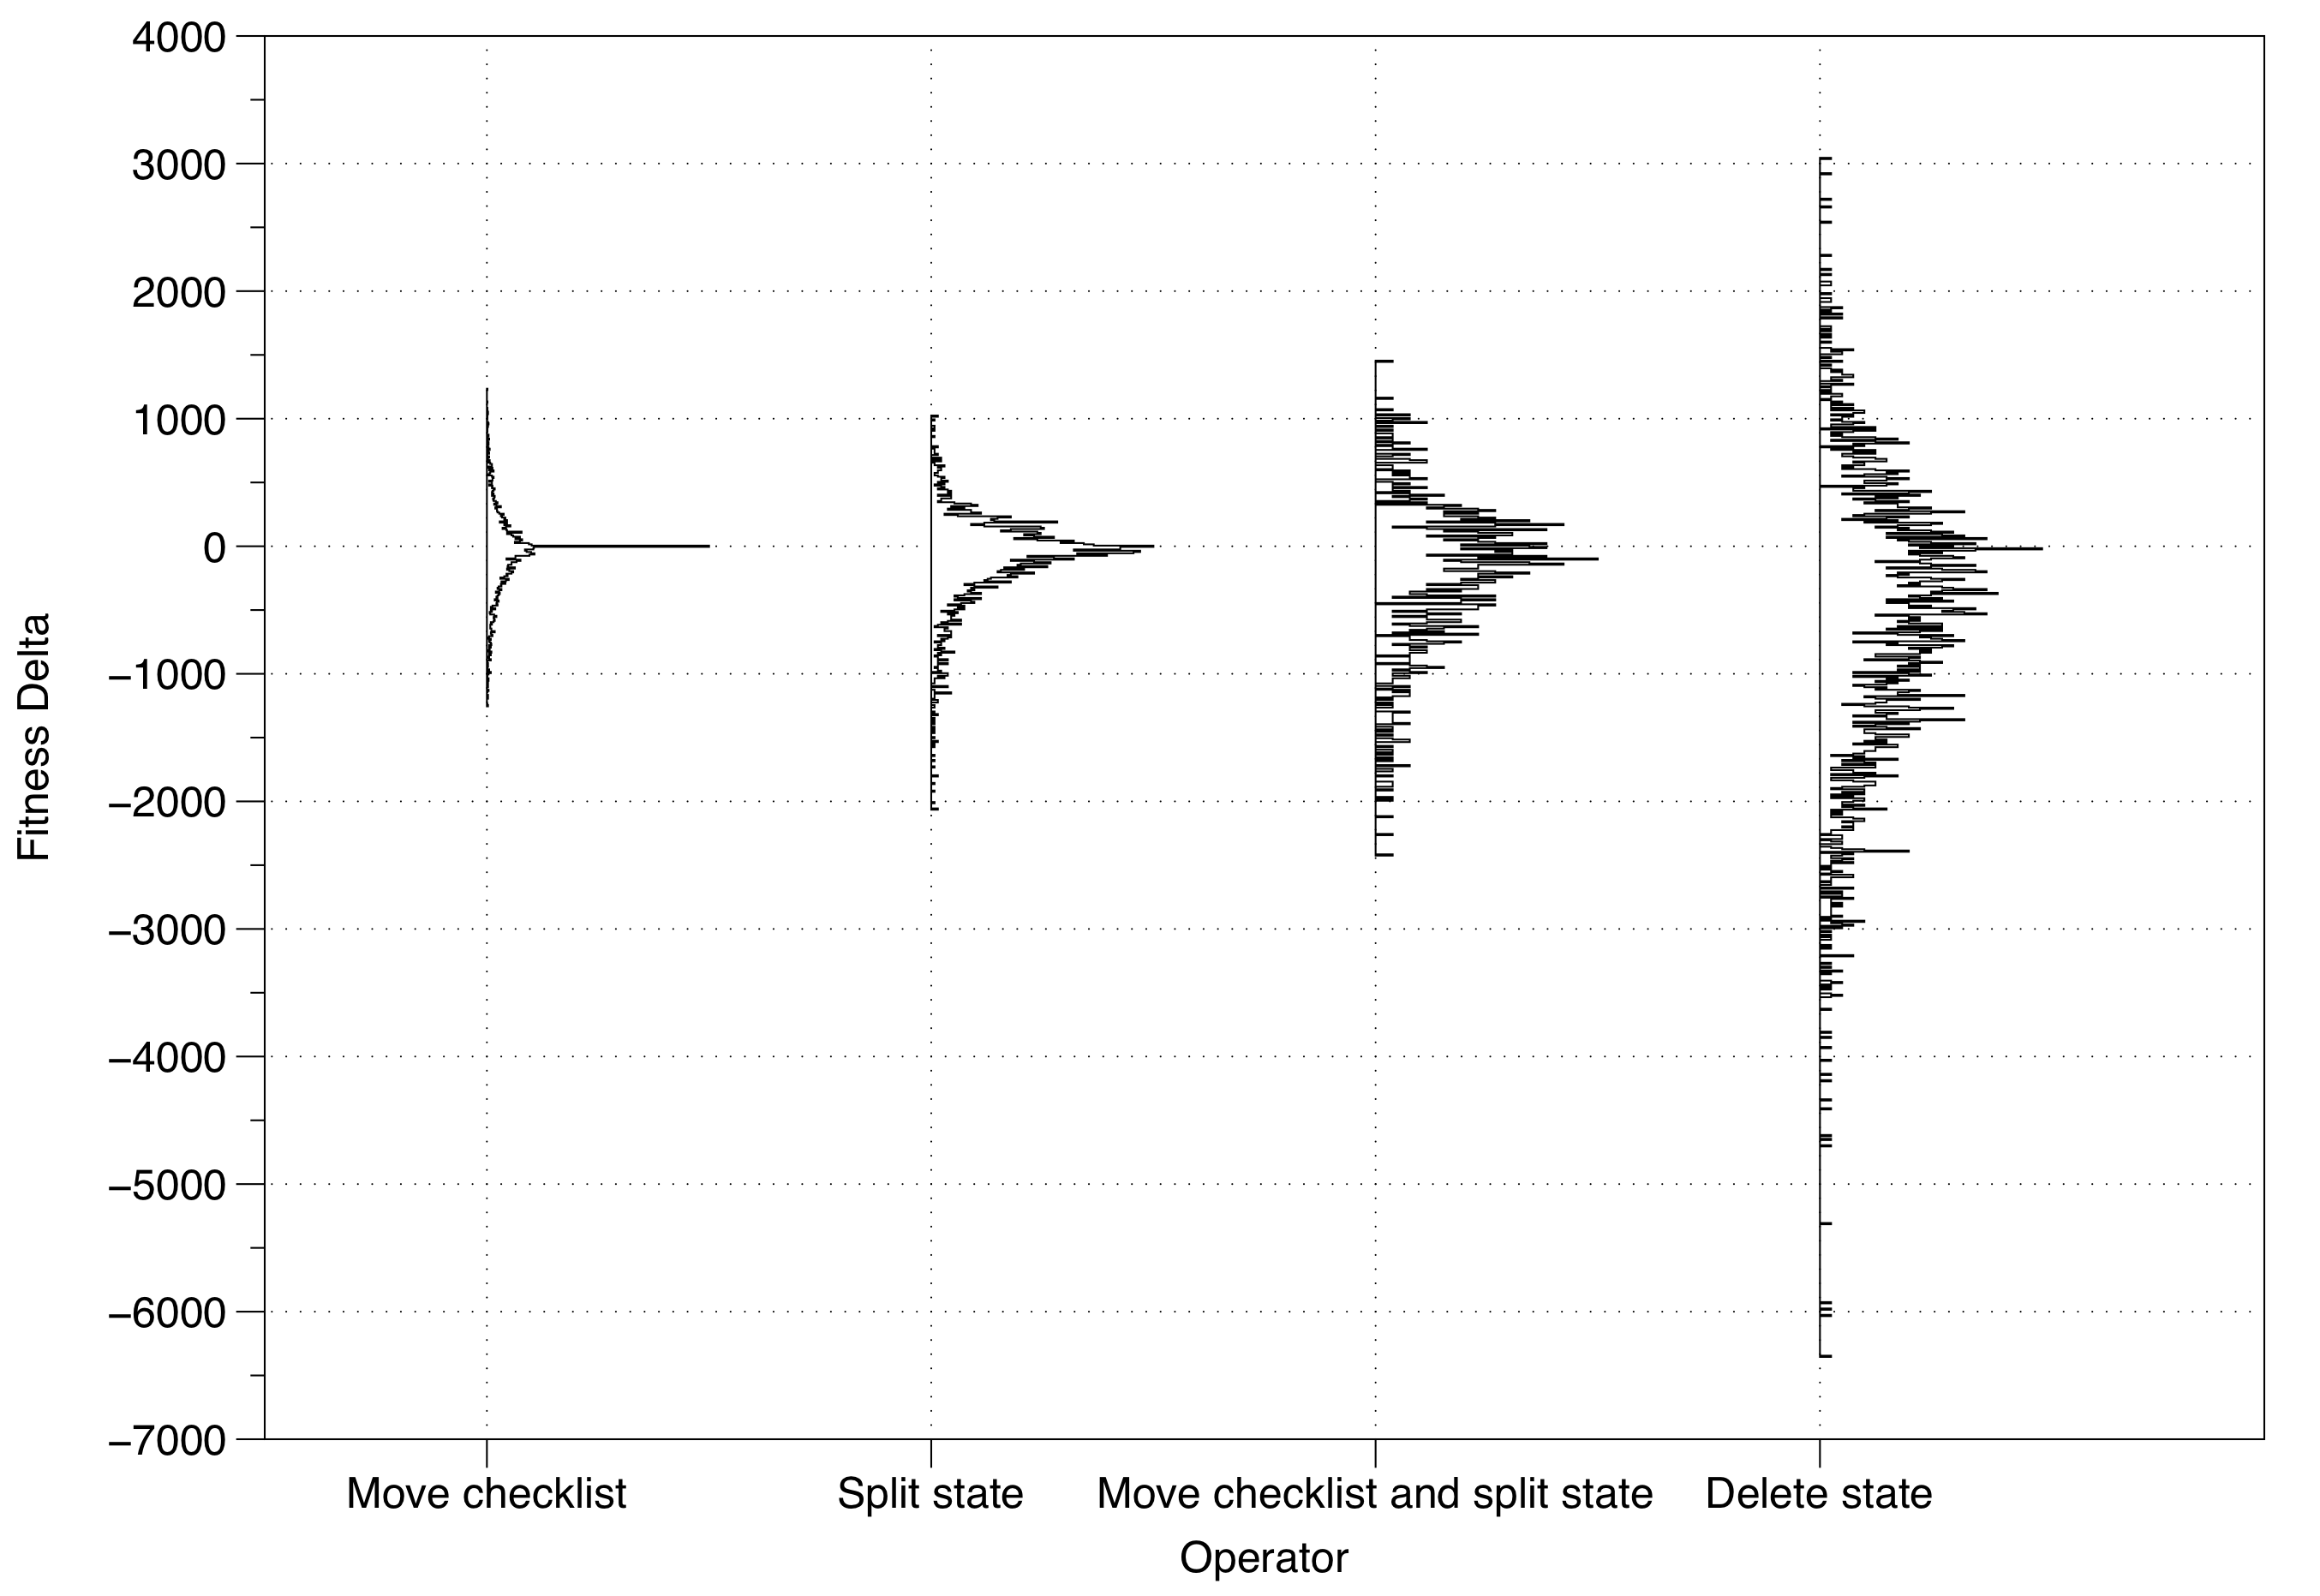
\includegraphics[scale=0.37]{images/operator_analysis_partial_order_first_5_gens}
\caption{Mutation Operators Effect on Fitness Scores for Partial Ordering}
\label{OperatorsPartialOrdering}
\end{figure}

\begin{itemize}
  \item ``move checklist" typically has the smallest impact on the fitness scores. Most of the distribution is tightly centered around zero. This operator is great for fine tuning a well established structure. 
  \item ``move checklist and split state" occurs when ``move checklist" adds a  checklist to a state that already has eight, causing an automatic split to happen. The distribution is similar to ``split state."
  \item ``split state" is a more ``destructive" operator to the data structure and has a wider range of impact than ``move checklist"
  \item ``delete state" causes the most change to the data structure and has the largest impact on fitness scores. 
\end{itemize}

The mean of all of these mutation operators is slightly negative. As with most genetic algorithms, applying any operator can cause a fitness score decrease and the offspring will eventually be discarded when the population surpasses it.

\subsection{How does the algorithm utilize states?}

Partial Ordering maintains a consistent number of states over time. Figure ~\ref{NumberOfStatesPartialOrdering} illustrates how a population utilizes the number of states when constrained to four alphas. The randomly created initial population ranges from 23 to 38 states and evolves to use roughly 25 to 30 states through out its generations. A stable number of states, as opposed to an infinitely growing number of states, is a desirable property for a fitness function. 

\begin{figure}[ht]
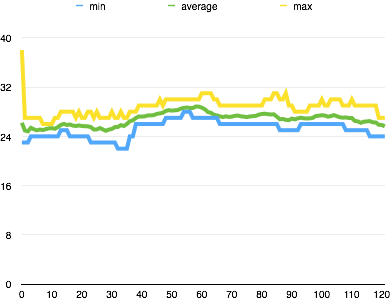
\includegraphics[scale=0.6]{images/number_of_states_partial_ordering}
\caption{Number of States Fitness Analysis for Partial Ordering}
\label{NumberOfStatesPartialOrdering}
\end{figure}

% The completion fitness function prefers to grow the kernel by adding more and more states.

\section{Best Generated Candidate Kernels}

Given the analysis from the previous section, namely that the Partial Ordering fitness function prefers smaller number of alphas, the best scoring candidates emerge quickly when starting with only a single alpha. Figure ~\ref{BestResultsPartialOrdering} shows the best, average, and worst fitness scores over 500 generations for 40 runs. (These 40 runs completed in 12.65 hours.) The graph also plots the fitness score of the original kernel.

The original kernel scores 13,372. The best generated kernel scores 85,122. For the Partial Ordering fitness function, the genetic algorithm had little difficulty in finding random solutions that score higher than the original kernel. The original kernel is optimized for human understanding and places 148 checklist items into logical sequences around themed alphas where as the candidate kernels are optimized around how teams actually flow through the checklist items.

\begin{figure*}[ht]
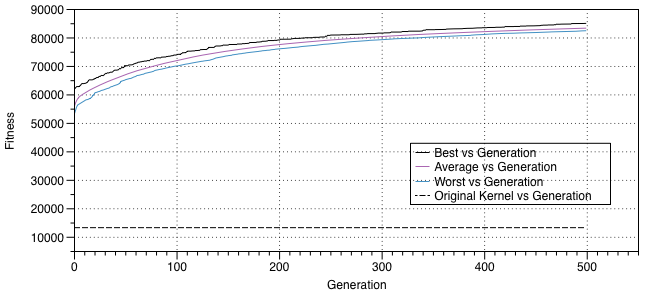
\includegraphics[scale=0.74]{images/best_results_partial_ordering_500gens_40runs}
\caption{Best Results for PartialOrdering}
\label{BestResultsPartialOrdering}
\end{figure*}

Table ~\ref{BestResults} shows the beginning two states for the final candidate which is a single alpha with 30 sequential states. The states contain a mixture of checklist items from different alphas. The candidate interweaves alphas into one flow based upon how teams accomplished the checklist items in practice. 

The generated kernel revealed that several checklists items that occur later in the original kernel often happen earlier on real projects. For example, the generated kernel places ``Team values stakeholders representatives' input" in the second state. Likewise, several checklist items that occur early in the original kernel often happen later on real projects. For example, the generated kernel places ``Defect levels are acceptable" in the second to last state. In future work, more analysis can be done with sufficient number of teams.

\begin{table}[h]
\caption{Highest Scoring Essence Kernel Generated By Genetic Algorithm}
\label{BestResults}
\centering
\begin{tabular}{|p{0.35in}|p{1.70in}|p{0.60in}|p{0.30in}|}
\hline
State & Checklist & Original \mbox{Alpha} & Original State \\ \hline
State 1 & Stakeholders wish to make an investment in better understanding potential value & Opportunity & 1. Identified \\ \hline
State 1 & User types are identified & Requirements & 1. Conceived \\ \hline
State 1 & Team agrees on relevant stakeholder groups to be represented & Stakeholders & 1. Recognized \\ \hline
State 1 & Representatives respect team's way of working  & Stakeholders & 2. Represented \\ \hline
State 2 & An idea for a software solution is identified & Opportunity & 1. Identified \\ \hline
State 2 & Funding model is clear & Work & 1. Initiated \\ \hline
State 2 & Stakeholder representatives agree to take on responsibilities & Stakeholders & 2. Represented \\  \hline
State 2 & Team values stakeholder representatives' input & Stakeholders & 4. In Agreement \\ \hline
State 2 & Opportunity addresses problem and stakeholder needs & Opportunity & 2. Solution Needed \\ \hline
\end{tabular}
\end{table}

% \section{Optimizing the Original Kernel}

% With the genetic algorithm code, we are able to optimize the existing kernel.

% To accomplish this, we utilized the following greedy algorithm: 
% First, iterate over the checklists and find the checklist item that would increase the fitness score the most if it was either moved forward or later. Second, move it. Third, repeat until there are no improvements in fitness score.

% The starting fitness score is 13,372 and it improves to 13,490 by moving 22 checklist items. In examining the final optimized kernel, several states can be combined. The \textbf{Stakeholder}'s \textit{Recognized} and \textit{Represented} states can be combined (Figure \ref{StakeholdersRecognized}). The \textbf{Team}'s \textit{Concluded} and \textit{Closed} states can be combined (Figure \ref{TeamConcluded}). From the empirical data, there is no clear distinction between these states as the states happen concurrently in practice.

% \begin{figure}[ht]
% 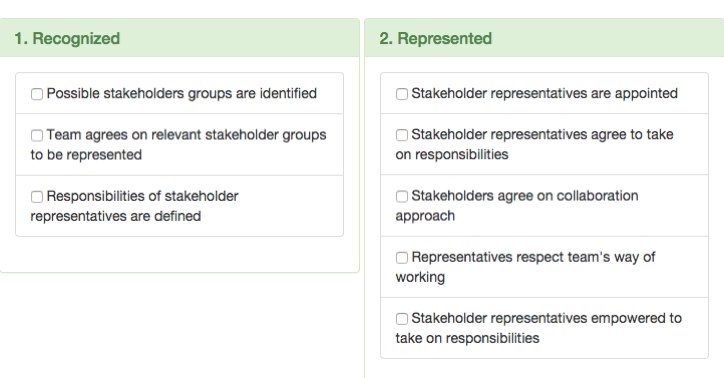
\includegraphics[scale=0.33]{kernel_images/stakeholders_1_2}
% \caption{Stakeholder's Recongized and Represented States Could be Combined}
% \label{StakeholdersRecognized}
% \end{figure}

% \begin{figure}[ht]
% 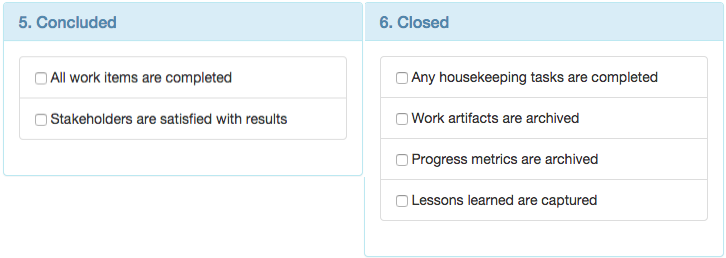
\includegraphics[scale=0.33]{kernel_images/team_5_6}
% \caption{Team's Concluded and Closed States Could be Combined}
% \label{TeamConcluded}
% \end{figure}

% The algorithm also revealed that several checklist items listed early in the original kernel often happen later on a real project:

% \begin{itemize}
% \item{\textbf{Opportunity}'s Desired outcomes are clear}
% \item{\textbf{Opportunity}'s Success criteria are clear}
% \item{\textbf{Software System}'s Selected architecture addresses key technical risks}
% \item{\textbf{Software System}'s Defect levels are acceptable}
% \end{itemize}

% If this is consistent with data from additional teams, then this suggests that these checklist items should be moved to a later state. 

\section{Threats to Validity}

\underline{Generalizability across situations}: the collected data is from faculty facilitating Essence Reflection meetings \cite{EASE2014} with masters of software engineering teams during their final practicum project at Carnegie Mellon University in Silicon Valley. This empirical data, and thus the results, may not represent teams in industry nor teams at other universities. Replicating the results from \cite{ICSE2014} would mitigate this threat.

\underline{Limited amount of empirical data}: the collected data is from five teams collecting data every week during the duration of a fifteen week semester. As a result, the generated solutions might be over-optimized to the empirical data. Collecting more data will diminish this threat. The purpose of this work is to show initial results in applying genetic algorithms for fitting possible candidate kernels to empirical data, not to recommend a replacement for the original Essence Kernel. 

\section{Conclusions and Future Work}

This paper describes how a genetic algorithm created random kernels using two different fitness functions. The candidate kernels have the same fundamental structure as the original Essence kernel: a collection of linear state machines called alphas with each state having a set of checklist items. 

We analyzed the genetic algorithm's search space. The Partial Ordering fitness function prefers smaller number of alphas and typically relies upon a stable number of states. Applying the ``delete state" mutation operator has the widest positive and negative effect on the resultant fitness score whereas the ``move checklist" and ``split state" have a narrower effect on fitness scores. 

The best generated random kernel scores higher than the original Essence kernel. 

Optimizations to the original Essence kernel are possible. Using the same code base, a greedy optimization algorithm altered the original Essence kernel and revealed that several states could be combined and several checklist items could move to better represent the empirical data collected so far.

As for next steps, collecting more empirical data will yield more reliable results and better insights. Future research includes considering an ALPS strategy \cite{ALPS} of age-based population pools. Given the mutation operator analysis on fitness, one strategy to consider is starting with operations that have large structural changes in younger populations, and then later optimizing checklists within a given structure. Additional research can experiment with how population size and weights of operators affect the genetic algorithm's performance. Additional experiments could consider altering the fitness function to have other desirable kernel properties such as limiting number of states or requiring a minimum number of alphas to be used.

In conclusion, genetic algorithms explore the kernel search space through random mutations. Given the human desire for order, the computer can consider solutions that people might immediately dismiss as not meeting certain aesthetic considerations. By considering these unusual solutions, the computer can further optimize the solution to achieve higher scoring candidate kernels. 


% Show this to Cecile

% \begin{table}[h]
% \caption{Starting State for Genetic Algorithms Like to Cheat}
% \label{CompletionCheatsInitial}
% \centering
% \begin{tabular}{|l|l|l|l|l|l|l|}
% \hline
% alpha 1 & 6 & 4 & 2 & 3 & 4 & 5 \\ \hline
% alpha 2 & 5 & 4 & 3 & 5 & 3 & 4 \\ \hline
% alpha 3 & 5 & 3 & 4 & 4 & 1 & 4 \\ \hline
% alpha 4 & 6 & 3 & 5 & 7 & 3 & 4 \\ \hline
% alpha 5 & 4 & 9 & 5 & 2 & 1 & 3 \\ \hline
% alpha 6 & 2 & 6 & 7 & 5 & 4 & 2 \\ \hline
% \end{tabular}
% \end{table}

% \begin{table}[h]
% \caption{Final State for Genetic Algorithms Like to Cheat}
% \label{CompletionCheatsFinal}
% \centering
% \begin{tabular}{|l|l|}
% \hline
% alpha 1 & 34 \\ \hline
% alpha 2 & 12 \\ \hline
% alpha 3 & 2  \\ \hline
% alpha 4 & 31 \\ \hline
% alpha 5 & 35 \\ \hline
% alpha 6 & 33 \\ \hline
% \end{tabular}
% \end{table}



% \begin{figure}[ht]
% 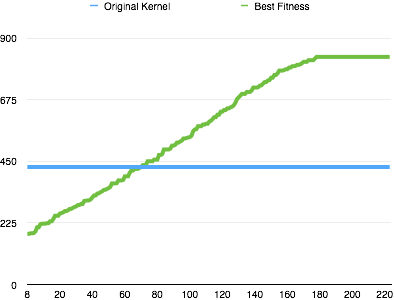
\includegraphics[scale=0.6]{images/initial_results_completion}
% \caption{Initial Results for Completion}\label{InitialResultsCompletion}
% \end{figure}

% \begin{figure}[ht]
% 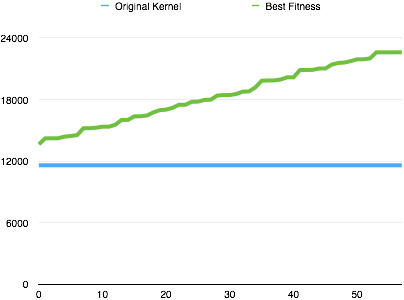
\includegraphics[scale=0.6]{images/initial_results_partial_ordering}
% \caption{Initial Results for PartialOrdering}\label{InitialResultsPartialOrdering}
% \end{figure}

% \begin{figure}[ht]
% 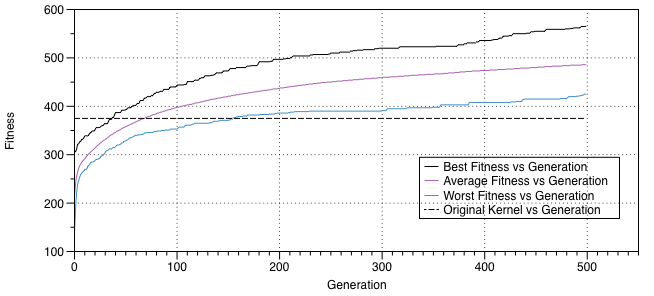
\includegraphics[scale=0.37]{images/best_results_completion_500gens_40runs}
% \caption{Best Results for Completion}\label{BestResultsCompletion}
% \end{figure}

% \begin{figure}[ht]
% 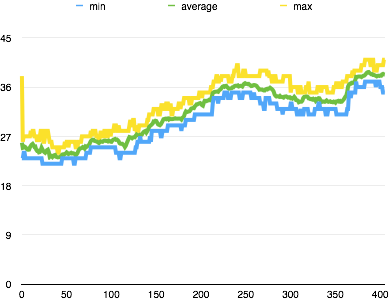
\includegraphics[scale=0.6]{images/number_of_states_completion}
% \caption{Number of States Fitness Analysis for Completion}\label{NumberOfStatesCompletion}
% \end{figure}

% \begin{figure}[ht]
% 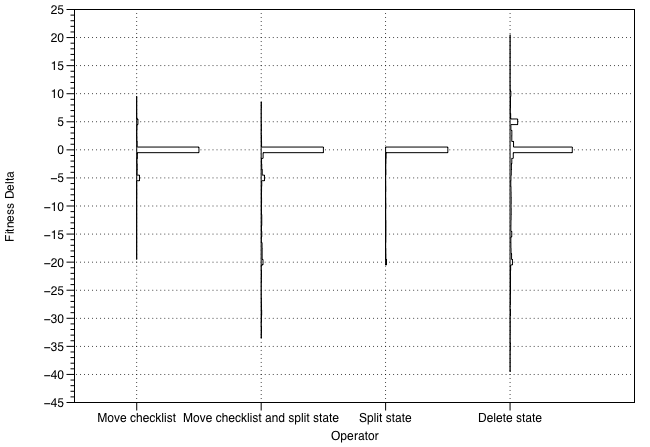
\includegraphics[scale=0.37]{images/operator_analysis_completion_first_5_gens}
% \caption{Mutation Operators Affect on Fitness Scores for Completion}\label{OperatorsCompletion}
% \end{figure}



% no \IEEEPARstart

% An example of a floating figure using the graphicx package.
% Note that \label must occur AFTER (or within) \caption.
% For figures, \caption should occur after the \includegraphics.
% Note that IEEEtran v1.7 and later has special internal code that
% is designed to preserve the operation of \label within \caption
% even when the captionsoff option is in effect. However, because
% of issues like this, it may be the safest practice to put all your
% \label just after \caption rather than within \caption.
%
% Reminder: the "draftcls" or "draftclsnofoot", not "draft", class
% option should be used if it is desired that the figures are to be
% displayed while in draft mode.
%
%\begin{figure}[!t]
%\centering
%\includegraphics[width=2.5in]{myfigure}
% where an .eps filename suffix will be assumed under latex,
% and a .pdf suffix will be assumed for pdflatex; or what has been declared
% via \DeclareGraphicsExtensions.
%\caption{Simulation Results}
%\label{fig_sim}
%\end{figure}

% Note that IEEE typically puts floats only at the top, even when this
% results in a large percentage of a column being occupied by floats.


% An example of a double column floating figure using two subfigures.
% (The subfig.sty package must be loaded for this to work.)
% The subfigure \label commands are set within each subfloat command, the
% \label for the overall figure must come after \caption.
% \hfil must be used as a separator to get equal spacing.
% The subfigure.sty package works much the same way, except \subfigure is
% used instead of \subfloat.
%
%\begin{figure*}[!t]
%\centerline{\subfloat[Case I]\includegraphics[width=2.5in]{subfigcase1}%
%\label{fig_first_case}}
%\hfil
%\subfloat[Case II]{\includegraphics[width=2.5in]{subfigcase2}%
%\label{fig_second_case}}}
%\caption{Simulation results}
%\label{fig_sim}
%\end{figure*}
%
% Note that often IEEE papers with subfigures do not employ subfigure
% captions (using the optional argument to \subfloat), but instead will
% reference/describe all of them (a), (b), etc., within the main caption.


% An example of a floating table. Note that, for IEEE style tables, the
% \caption command should come BEFORE the table. Table text will default to
% \footnotesize as IEEE normally uses this smaller font for tables.
% The \label must come after \caption as always.
%
%\begin{table}[!t]
%% increase table row spacing, adjust to taste
%\renewcommand{\arraystretch}{1.3}
% if using array.sty, it might be a good idea to tweak the value of
% \extrarowheight as needed to properly center the text within the cells
%\caption{An Example of a Table}
%\label{table_example}
%\centering
%% Some packages, such as MDW tools, offer better commands for making tables
%% than the plain LaTeX2e tabular which is used here.
%\begin{tabular}{|c||c|}
%\hline
%One & Two\\
%\hline
%Three & Four\\
%\hline
%\end{tabular}
%\end{table}


% Note that IEEE does not put floats in the very first column - or typically
% anywhere on the first page for that matter. Also, in-text middle ("here")
% positioning is not used. Most IEEE journals/conferences use top floats
% exclusively. Note that, LaTeX2e, unlike IEEE journals/conferences, places
% footnotes above bottom floats. This can be corrected via the \fnbelowfloat
% command of the stfloats package.


% conference papers do not normally have an appendix


% use section* for acknowledgement





% trigger a \newpage just before the given reference
% number - used to balance the columns on the last page
% adjust value as needed - may need to be readjusted if
% the document is modified later
%\IEEEtriggeratref{8}
% The "triggered" command can be changed if desired:
%\IEEEtriggercmd{\enlargethispage{-5in}}

% references section

% can use a bibliography generated by BibTeX as a .bbl file
% BibTeX documentation can be easily obtained at:
% http://www.ctan.org/tex-archive/biblio/bibtex/contrib/doc/
% The IEEEtran BibTeX style support page is at:
% http://www.michaelshell.org/tex/ieeetran/bibtex/
%\bibliographystyle{IEEEtran}
% argument is your BibTeX string definitions and bibliography database(s)
%\bibliography{IEEEabrv,../bib/paper}
%
% <OR> manually copy in the resultant .bbl file
% set second argument of \begin to the number of references
% (used to reserve space for the reference number labels box)
% \begin{thebibliography}{1}

% \bibitem{IEEEhowto:kopka}
% H.~Kopka and P.~W. Daly, \emph{A Guide to \LaTeX}, 3rd~ed.\hskip 1em plus
%   0.5em minus 0.4em\relax Harlow, England: Addison-Wesley, 1999.

% \end{thebibliography}

\bibliographystyle{IEEEtran}
\bibliography{bibliography}


% that's all folks
\end{document}


